\documentclass[a4paper, 12pt]{article}
\usepackage{listings}
\usepackage{xcolor}
\usepackage{tikz}

% Pseudocode settings
\lstset{
    language=Python,
    basicstyle=\ttfamily,
    keywordstyle=\color{blue},
    commentstyle=\color{green},
    stringstyle=\color{red},
    frame=single,
    breaklines=true
}

\title{Lesson Notes}
\author{Your Name}
\date{\today}

\begin{document}

\maketitle

\section{Mathematics}
% Add your math content here
Here is an example of a mathematical equation:
\[
    E = mc^2
\]

You can also include inline math:
The Pythagorean theorem states that \( a^2 + b^2 = c^2 \).

\subsection{Example Diagram}
% Example TikZ diagram
\begin{center}
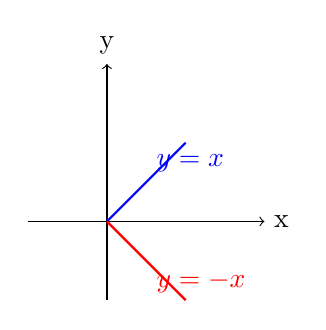
\begin{tikzpicture}
    \draw[->] (-1,0) -- (2,0) node[right] {x};
    \draw[->] (0,-1) -- (0,2) node[above] {y};
    \draw[thick, blue] (0,0) -- (1,1) node[midway, above right] {$y = x$};
    \draw[thick, red] (0,0) -- (1,-1) node[midway, below right] {$y = -x$};
\end{tikzpicture}
\end{center}

\section{Pseudocode}
% Add your pseudocode here
\begin{lstlisting}
# Example of a simple algorithm
function exampleAlgorithm(input):
    if input > 0:
        return "Positive"
    else:
        return "Non-positive"
\end{lstlisting}

\section{Additional Notes}
% Use this section for any extra notes
Here you can add any other relevant information or remarks about the lesson.

\end{document}
